\section{Introduction} \label{introduction}
\begin{sectionplan}
     \begin{itemize}
          \item  General introduction about how important compilers are and how
                 everyone and is using them in some form or another.

          \item Talk about research into parallel compilers at a highlevel,
                ie the current state of research, when research has been done,
                parallel compilers historically of low importance.

          \item Justify further research into compilers based on their use
                in software development and other fields.

          \item Link to next section that describes how compilers work at a
                high level
     \end{itemize}
\end{sectionplan}

Compilers are an important part of the interface between a programmer and the
computer for which he is developing software. The modern software ecosystem
could not exist without the frequent and extensive use of compilers in the
software development process. It is of no surprise that the study of compilers
and programming languages has been an important field of research in computer
science for many decades. Any improvements in compiler technology can have wide
and long lasting affects on software development \citep{hall_compiler_2009}.

The focus of my FYP is to study a subset of compiler research regarding parallel
compilation. Research into this niche has been historically of low priority.
Traditional compiler architecture since the 1970’s was focused on minimising
memory use and optimising for single threaded performance (\textbf{citation
needed}). This was at a time when computers didn’t even have enough ram to store
all the data necessary for compiling large amounts of source code.  Commodity
hardware has since improved significantly. The memory available in a computer
is much more abundant than before and single threaded processor speed is not
improving at the same rate as it once did (\textbf{citation needed}). In fact,
were seeing commodity processors contain many cores capable of running dozens of
threads in parallel. I believe this is sufficient cause to consider alternative
architectures that better utilise this environment.

Modern compiler implementations in use today often use varying amounts of
parallelism in order to speed up compilation times. The rustc compiler team
reports that the time spent in the compiler frontend of the rustc compiler
was reduced by 50\% after increasing the amount of work it does in parallel.
\citep{nicholas_nethercote_faster_2023}. Improvements are not limited to
the compiler frontend. The mold linker project boasts significantly better
performance than its competitors due to its extensive and clever use of
parallelism \citep{rui_ueyama_design_nodate}. The potential for performance
improvements is clearly evident in modern compilers. Moreover, compiler research
and development can generalize to other areas outside of software development.

Applications of techniques traditionally associated with compilers
can be found in network packet parsing \citep{wang_hyperscan_2019,
roesch_snort_1999} and huffman decoding \citep{howard_parallel_1996}.
These areas, among others, can benefit from research directed at improving
compiler technology due to a significant overlap in the underlying theory
\citep{mytkowicz_data-parallel_2014}. Futher development in compiler theory can
be justified not only by its direct benefit to software development but also its
affect on tangential fields of research.

The next section describes the sequential method of compilation which can be
seen in a large number of compilers.

\subsection{Sequential Compilation}
\begin{sectionplan}
     Short explanation of compiler technology and the structure of a compiler.
     Explain the compilation process and the use cases for compilation.
\end{sectionplan}

\begin{figure}[t]
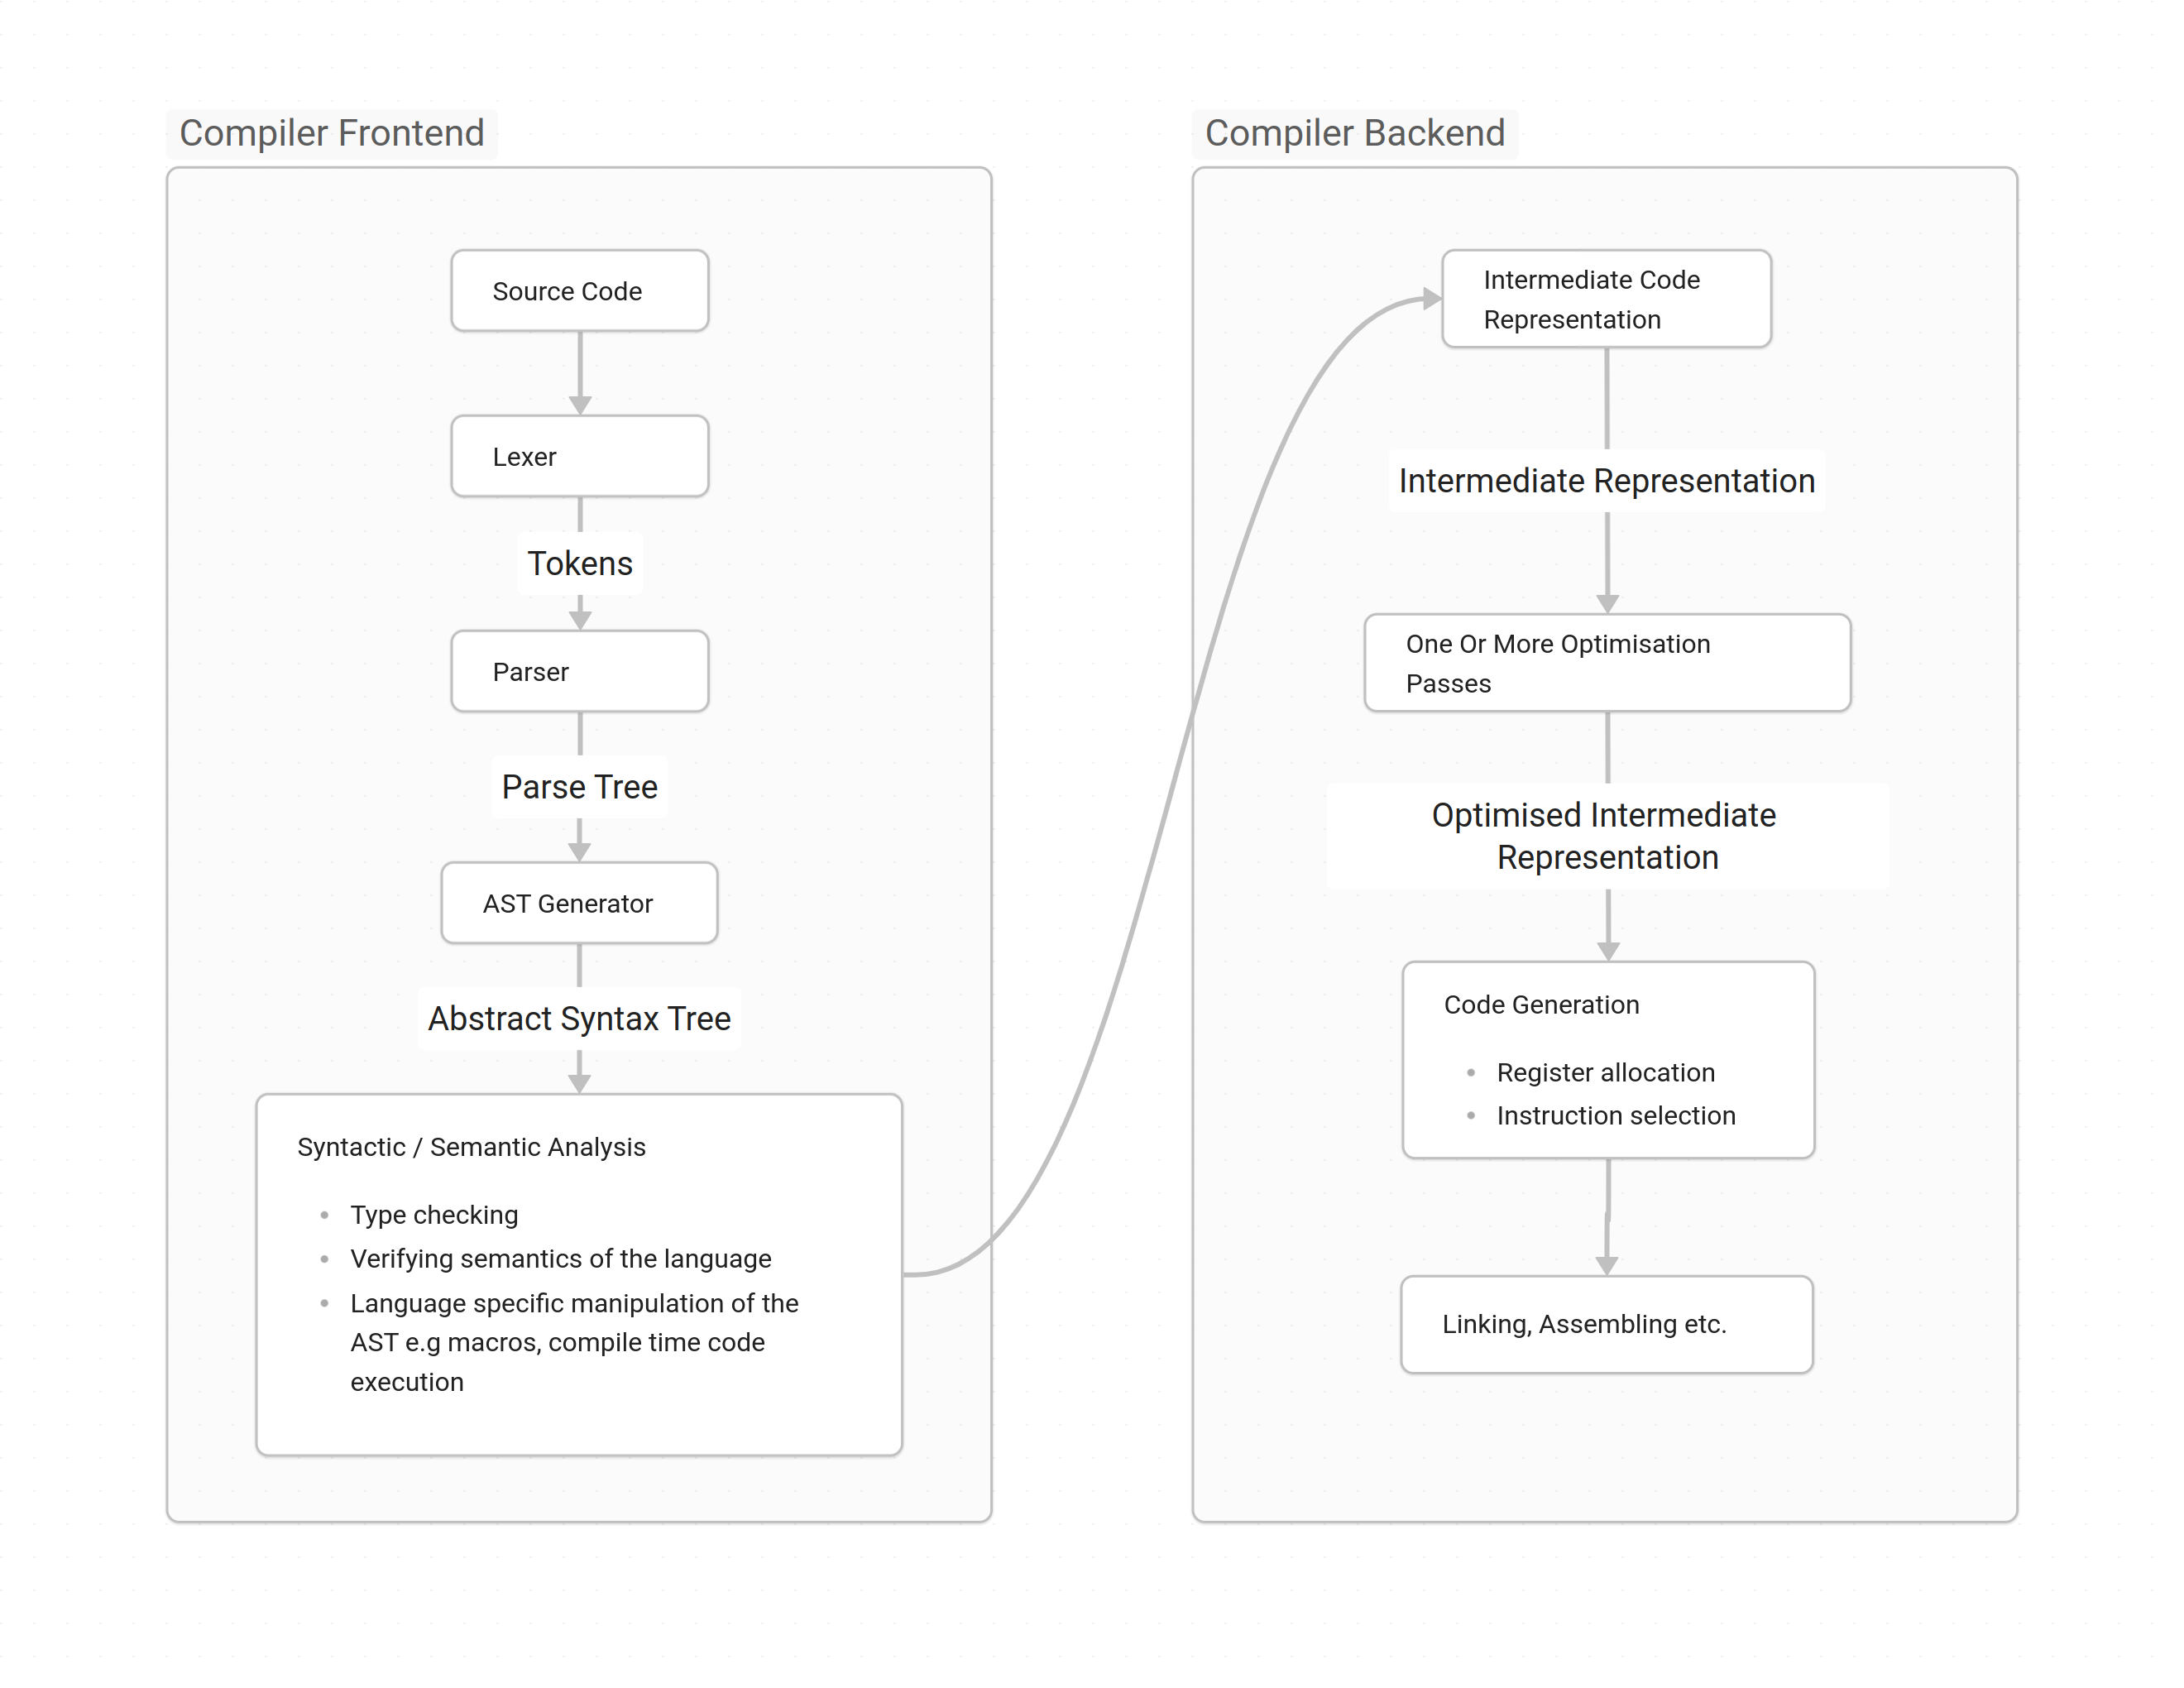
\includegraphics[width=\linewidth]{images/generic_compiler.png}
\centering
\caption{Compilation phases in a generic compiler}
\label{fig:compiler}
\end{figure}

The function of a compiler is to transform source code from one language into
another. During this process, a compiler will usually lose information in the
source code that is useful to the programmer but useless to the machine that
will execute the program. Inside a compiler, the source code passes through
several algorithms that transform the code in various ways. These different
compilation stages are visualised in figure \ref{fig:compiler}.

Compilers work in a sequential way that resemebles a pipeline. The lexer splits
up the source code into words called tokens. The parser then takes those tokens
and assigns structure to them by arraging them as a graph. This structure makes
them easier to meaningfully navigate. It addtionally lets the tokens better describe
what they mean, beyond what can be understood from a simple list of words. This
graph of tokens is then analysed during the semantic analysis phase, doing
things like looking for unsused variables. The parts of the compiler up to this
point are colloquially called the frontend of the compiler.

The stages of a compiler that are reponsible for taking a file from
source code to code generation are often implemented with little to no
parallelisation(\textbf{citation needed}). An example of going from source
code to machine code is the process of compiling a C file into an object file.
As can be seen from figure \ref{fig:compiler}, this envelopes a significant
portion of the compiler. 

\subsection{Parallel Compiliation}
\begin{sectionplan}
	What is meant by parallel compilation?
\end{sectionplan}


\subsubsection{Advantages Of Parallel Compilation}
\begin{sectionplan}
     Reasons why parallel compilation is good / better compared to sequential
	 compilation.

     \begin{itemize}
          \item More cores used during compilation increase compiler performance
                and better overall system usage

          \item Hardware investments in the industry involve specialisation
                and increasing reliance on performance gained from parallel
                architectures. Existing compilers cannot benefit from this.

          \item Choosing a language syntax as a language designer based on how
                well it can be processed in parallel in the future is necessary
                early on. Making those choices is difficult due to a lack of
                research.
     \end{itemize}
\end{sectionplan}

Using multiple CPU cores during compilation can speed up compilation time.
Researchers in 2009 created an optimised lexer for a machine that had a large
number of cores that could run code in parallel
\citep{scarpazza_high-performance_2009}. It had eight cpu cores where each core
could run eight threads in parallel for a total of 64 parallel threads.  This
shows how using parallel processing to speed up compilation tasks is not a new
idea. Subsequent research into parallel lexing from 2014 achieved a 14 times
speed up for lexing HTML on a 16 core system
\citep{mytkowicz_data-parallel_2014}. Substantial performance gains can clearly
be achieved through parallelisation.

There have been increasingly larger investments in the hardware industry for
specialised hardware beyond the typical CPU. Examples include things like smart
nics that offload network packet parsing from the CPU or DPU’s that provide
more facilities for networking and input / output related tasks than a typical
CPU. A recent article from October 2023 shows how AMD’s software stack for
general purpose computing on graphics cards known as rocm is now among their
top priorities \citep{ward-foxton_rocm_2023}. As time goes on, we are likely
to see increasingly specialised and heterogenous hardware (\textbf{citation
needed}). Traditional compiler architecture is not well suited to this type
of environment.

For many programming languages, once a syntax goes into general use, it becomes
nearly impossible to revert or change it in a way that breaks existing programs.
This leads to programming languages becoming complicated and hard to define as
new features are added. For example, langauges like C++ are extremely hard to
compile in any way, let alone a parallel way. Research into and the development
of parallel compilers can aid future developers when they are choosing their
syntax or what features they want to implement without making their language
hard to compile in parallel (\textbf{citation needed}). It is currently
rather difficult to design a language that can easily be compiled in parallel
due to a lack of research and prior work compared to sequential approaches
(\textbf{citation needed}).

\subsubsection{Fine-Grained Parallel Compilation}
\begin{sectionplan}
	Justify looking at alternative forms of parallelism besides the status quo 	
	method of compiling source files in parallel and linking them together in the
	end.

	\begin{itemize}
     	\item Finer grained parallelism is better suited for running code on 				
			  massively parallel hardware like GPU's.

     	\item Error handling potential improved by being able to independantly
			  process any part of text. No need for complex parser recovery.

     	\item More parts of a program can be compiled in parallel which makes
			  better use of a computers parallel processing facilities. Mention 
			  ahmdals law.

     	\item (weak) Reduced bottle neck when compiling very large files (since 			
			  individual files are split up and compiled in parallel).

		\item Significant speedups in other fields where only one stage of is 
			  needed like lexing and parsing very large amounts of structured 
			  data. Mention PAPAGENO parser with relation to simdjson.
	\end{itemize}
\end{sectionplan}

Many existing compilers can operate in parallel by compiling several source
code files at the same time. In this work I am looking at methods employing
finer-grained parallelism where various stages of a compiler can be executed
in parallel.

\subsection{Objectives of My Work}

The goal of my project is to research ways of the compilation stages in
a compiler frontend by using parallel processing methods, aswell as an
implementation of those stages if time allows.

\subsection{Structure of Report}

Chapter \ref{introduction} provides an introduction to parallel compilation as
well as reasons for continued effort in this area of research.
\newline \newline
Chapter \ref{litreview} describes exisiting approaches for compiling
in parallel.
\newline \newline
Chapter \ref{design} elaborates on the issues associated with designing a
parallel compiler aswell as the design of my compiler implementation. I discuss
the various approaches mentioned in the literature review, including their
advantages and disadvantages where appropriate.
\newline \newline
Chapter \ref{implementation} explains the details of my implementation,
referring to things like external code dependancies and program structure.
\newline \newline
Chapter \ref{evalandtesting} describes my testing methodologies and the evaluation of my compilers performance.
\newline \newline
Chapter \ref{conclusion} concludes the report with a summary of the report and
concluding remarks.
